% PathoFluor-At manuscript.
% Every number in the text is a macro from numbers.tex, generated by ../scripts/07_numbers.py
% from ../tables/ and ../metadata/. Methods facts trace to ../metadata/FACTS_PENDING.md.
% references.bib is generated from Crossref records by ../scripts/make_bib.py.
% \pending{...} marks facts or results not yet available; the draft PDF shows them in red.

\documentclass[11pt,a4paper]{article}
\usepackage[utf8]{inputenc}
\usepackage[T1]{fontenc}
\usepackage{lmodern}
\usepackage[margin=2.4cm]{geometry}
\usepackage{graphicx}
\usepackage{booktabs}
\usepackage{amsmath}
\usepackage{xcolor}
\usepackage[hidelinks]{hyperref}
\usepackage[numbers,sort&compress]{natbib}
\usepackage{authblk}
\usepackage[font=small,labelfont=bf]{caption}
\usepackage{microtype}
\usepackage{lineno}
\usepackage{textcomp}
\graphicspath{{../figures/}}
\linenumbers
% Generated by scripts/07_numbers.py from tables/ and metadata/. Do not edit by hand.
\newcommand{\nFiles}{7,752}
\newcommand{\nCubes}{400}
\newcommand{\nCubesA}{216}
\newcommand{\nCubesB}{168}
\newcommand{\nRoiFiles}{5,842}
\newcommand{\nRoiUnique}{2,486}
\newcommand{\nRoiA}{1,982}
\newcommand{\nRoiB}{504}
\newcommand{\rawGB}{396}
\newcommand{\rawFzero}{2,588}
\newcommand{\rawFone}{2,044}
\newcommand{\rawDropPct}{21}
\newcommand{\cpsDiffPct}{4}
\newcommand{\satHzeroMaxPct}{13}
\newcommand{\satHzeroMedPct}{0.1}
\newcommand{\pathFwhmOneSD}{2.07}
\newcommand{\pathFwhmOnenm}{1.40}
\newcommand{\pathFwhmOneq}{0.018}
\newcommand{\pathFwhmTwoSD}{2.39}
\newcommand{\pathFwhmTwonm}{1.76}
\newcommand{\pathFwhmTwoq}{6.8\times10^{-4}}
\newcommand{\pathSwTwoSD}{1.77}
\newcommand{\pathSwTwoq}{0.018}
\newcommand{\pathFwhmThreenm}{1.02}
\newcommand{\pathFwhmThreeq}{0.005}
\newcommand{\pathSwThreeSD}{2.03}
\newcommand{\pathSwThreeq}{6.9\times10^{-4}}
\newcommand{\pathFwhmTwentyFournm}{3.35}
\newcommand{\pathFwhmTwentyFourq}{0.005}
\newcommand{\pathSwTwentyFourSD}{2.46}
\newcommand{\pathSwTwentyFourq}{4.3\times10^{-5}}
\newcommand{\cmlFourSwSD}{-1.74}
\newcommand{\cmlFourSwq}{0.036}
\newcommand{\flgFwhmThreeSD}{2.18}
\newcommand{\flgFwhmThreeq}{0.005}
\newcommand{\nBaselineTests}{270}
\newcommand{\nBaselineSig}{13}
\newcommand{\hzeroFlgFwhmSD}{-1.29}
\newcommand{\hzeroFlgFwhmq}{5.5\times10^{-5}}
\newcommand{\setBinterSD}{1.78}
\newcommand{\setBinterq}{0.026}
\newcommand{\setBinterN}{4}
\newcommand{\aucPathOne}{1.00}
\newcommand{\pPathOne}{0.029}
\newcommand{\aucPathTwo}{1.00}
\newcommand{\pPathTwo}{0.029}
\newcommand{\aucPathTwentyFour}{1.00}
\newcommand{\pPathTwentyFour}{0.029}
\newcommand{\aucPathThree}{0.75}
\newcommand{\pPathThree}{0.143}
\newcommand{\aucPlaceboFlg}{1.00}
\newcommand{\pPlaceboFlg}{0.029}
\newcommand{\aucPlaceboPath}{0.81}
\newcommand{\aucFlgEarlyMin}{0.89}
\newcommand{\aucFlgEarlyMax}{1.00}
\newcommand{\pFlgEarlyMin}{0.10}
\newcommand{\nPermFlgBase}{20}
\newcommand{\specFlgColO}{0.18}
\newcommand{\specFlgFlsSeventeen}{0.36}
\newcommand{\specFlgFlsOneOhOne}{0.24}
\newcommand{\nUseSubset}{1,358}
\newcommand{\nCopyFiles}{16}
\newcommand{\nOffsetRoi}{83}
\newcommand{\offsetMedian}{109}
\newcommand{\offsetCleanMedian}{0.1}
\newcommand{\nKeyConflict}{12}
\newcommand{\nTagValues}{25}

\newcommand{\pending}[1]{\textcolor{red}{[PENDING: #1]}}

\title{\bfseries Fluorescence hyperspectral imaging detects an early, FLS2-independent
signature of \textit{Pseudomonas syringae} challenge in \textit{Arabidopsis} seedlings,
but not of flg22 perception}
\author[1]{Richard J. Barker\thanks{ORCID 0000-0001-5681-9857. Correspondence: richard@cosecloud.com}}
\author[ ]{\pending{co-authors and affiliations (FACTS P10)}}
\affil[1]{\pending{affiliation}}
\date{\pending{date}}

\begin{document}
\maketitle

\begin{abstract}
\noindent
Detecting plant infection before symptoms appear would help both field and
controlled-environment agriculture. In 2016 we imaged \textit{Arabidopsis} seedlings by
fluorescence hyperspectral imaging (488\,nm excitation, 500--800\,nm emission) before and
1--48\,h after treatment with a mock solution, the flagellin epitope flg22 or
\textit{Pseudomonas syringae}. Five genotypes were imaged: Col-0, two \textit{fls2} receptor
mutants and two \textit{cml24} Ca$^{2+}$-sensor mutants. We reanalysed all \nRoiA{} hand-drawn
seedling spectra of the primary experiment, and \nCubes{} raw image cubes (\rawGB{}\,GB).
Recovering the camera metadata showed that exposure time changed between timepoints: the
2016 summaries' \rawDropPct{}\% fall in intensity after treatment disappears (to within
\cpsDiffPct{}\%) once intensities are divided by exposure. Treated and control plates also
differed \emph{before} treatment, enough for a classifier to tell them apart (plate-level
AUC \aucPlaceboFlg{}), so we analysed only change from each plate's own baseline.
On that basis, \textit{P.~syringae} broadened the red chlorophyll emission peak within 1\,h
(+\pathFwhmOnenm{}\,nm; $q=\pathFwhmOneq$). By 2\,h it had also raised emission below
640\,nm, and change-from-baseline spectra separated infected from control plates perfectly
at 1, 2 and 24\,h (leave-plate-out AUC \aucPathTwo{}; exact permutation $p=\pPathTwo$).
The pathogen signature appeared in every genotype. A flg22 signal was weaker
(AUC \aucFlgEarlyMin--\aucFlgEarlyMax{}, $p\geq\pFlgEarlyMin$). It was as strong in both
\textit{fls2} mutants, which cannot perceive flg22, as in Col-0, so in this experiment it
reflects a plate-level effect rather than flg22 perception. We release the raw data,
manifests, code and a reproducible pipeline as a FAIR resource, and document every data
problem we found.
\end{abstract}

\section{Introduction}
Plants perceive bacteria through pattern-recognition receptors long before disease
symptoms appear. The best-characterised receptor is FLS2, which binds the conserved flg22
epitope of bacterial flagellin \citep{felix1999,gomezgomez1999,gomezgomez2000,chinchilla2006}.
flg22 induces defence-gene expression and resistance in wild-type plants but not in
\textit{fls2} mutants. \textit{fls2} plants still respond to bacterial extracts through other
patterns, and are more susceptible to \textit{P.~syringae} pv.\ tomato DC3000 sprayed on the
leaf surface \citep{zipfel2004}. Pattern-triggered defence quickly lowers non-photochemical
quenching \citep{gohre2012}. \textit{P.~syringae} infection changes photosynthetic chlorophyll
fluorescence parameters near the infection site before visible symptoms, within 3\,h for an
avirulent strain \citep{bonfig2006}. Chlorophyll fluorescence imaging is therefore a
candidate for disease detection and phenotyping
\citep{rousseau2013,perezbueno2016,perezbueno2019,mahlein2016}.

Steady-state chlorophyll fluorescence emission has two bands, near 685--690\,nm and
730--740\,nm. Because chlorophyll reabsorbs the red band, their ratio falls as chlorophyll
content rises. The ratio also depends on leaf structure, optics and photosynthetic activity
\citep{buschmann2007}. Fluorescence hyperspectral imaging records the whole emission spectrum
at every pixel, so subtle shape changes can be mapped, not just one or two ratios.

\textit{CML24} (\textit{TCH2}) encodes a calmodulin-like Ca$^{2+}$ sensor whose transcript is
induced by touch, darkness and other stimuli \citep{delk2005}. The \textit{cml24-4} mutant is
impaired in pathogen- and pattern-induced nitric-oxide production \citep{ma2008}. This makes
CML24 a candidate link between early Ca$^{2+}$ signalling and downstream changes visible in
fluorescence.

Here we reanalyse a 2016 experiment designed to ask whether bacterial challenge and flg22
perception leave a hyperspectral fluorescence signature, and whether that signature
depends on FLS2 or CML24. Its fls2 mutants supply the key control: an flg22 signature that
reflects perception should be absent in them.

\section{Results}

\subsection{Recovering the experiment from its raw files}
We inventoried \nFiles{} files and parsed every file name into a design record, with no
exceptions. That gave \nCubesA{} sample cubes for the primary July experiment (set A),
\nCubesB{} for an independent November replicate (set B) and \nRoiFiles{} hand-drawn ROI
spectra (\nRoiUnique{} unique by content). The headers revealed that exposure changed between
timepoints (Fig.~\ref{fig:exposure}a). The 2016 graphs plotted raw counts, so their drop in
Control intensity from \rawFzero{} to \rawFone{} counts after hour~0 (Fig.~\ref{fig:exposure}b)
is largely a camera setting. Exposure-corrected Control intensities at 1--3\,h lie within
\cpsDiffPct{}\% of hour~0 (Fig.~\ref{fig:exposure}c). Hour-0 scans also saturated the 12-bit
detector in up to \satHzeroMaxPct{}\% of a cube's seedling pixels (median \satHzeroMedPct{}\%).
We therefore based the primary analysis on exposure-independent shape features.

\begin{figure}[t]\centering
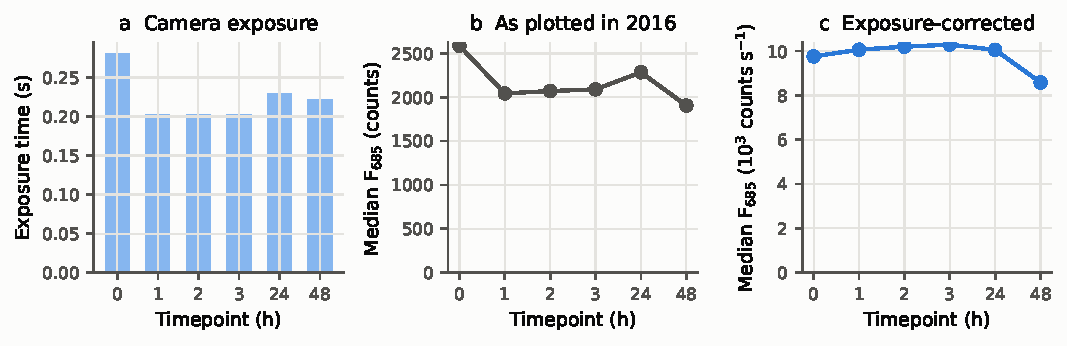
\includegraphics[width=\linewidth]{fig1_exposure_artefact.pdf}
\caption{\textbf{The 2016 intensity drop after treatment is an exposure artefact.}
(a) Exposure time per timepoint (plate mean, Control plates). (b) Median 683--687\,nm emission of
Control hand ROIs as plotted in 2016 and (c) divided by exposure. Data:
\texttt{results/roi\_spectra\_A.parquet}, \texttt{metadata/cube\_manifest.csv}.}
\label{fig:exposure}
\end{figure}

\subsection{Plates differed before treatment}
Hour~0 was imaged before treatment (as the scan times and the 2016 vendor report indicate; FACTS R6,
P13). Even so, flg22 plates already differed from Control plates
in red-peak width ($\hzeroFlgFwhmSD$\,SD; $q=\hzeroFlgFwhmq$). A classifier separated them
perfectly from spectra alone (plate-level AUC \aucPlaceboFlg{}, $p=\pPlaceboFlg$;
Fig.~\ref{fig:auc}a). The same held, less strongly, for Pathogen plates (AUC \aucPlaceboPath{}).
Plate-to-plate differences in seedling batch, placement or imaging geometry are thus as large as
the effects we want to detect. All inference below uses change from each plate's own hour-0
baseline, with the plate as the experimental unit.

\subsection{An early pathogen signature}
Relative to baseline, \textit{P.~syringae} broadened the red emission peak of Col-0 seedlings
by \pathFwhmOnenm{}\,nm at 1\,h ($\pathFwhmOneSD$\,SD, $q=\pathFwhmOneq$) and \pathFwhmTwonm{}\,nm
at 2\,h ($\pathFwhmTwoSD$\,SD, $q=\pathFwhmTwoq$). It also raised the 500--640\,nm fraction of
emission at 2\,h ($\pathSwTwoSD$\,SD, $q=\pathSwTwoq$; Figs~\ref{fig:spectra},~\ref{fig:time}).
These were the only \nBaselineSig{} of \nBaselineTests{} baseline-adjusted tests significant at
$q<0.05$. The spectral change deepened through 24\,h (Fig.~\ref{fig:spectra}a). A classifier on
change-from-baseline spectra separated infected from control plates perfectly at 1, 2 and 24\,h
(AUC \aucPathOne, \aucPathTwo, \aucPathTwentyFour; exact $p=\pPathOne$ each, close to the
smallest $p$ the 70 plate relabellings allow; Fig.~\ref{fig:auc}b). It failed at 3\,h
\pending{explain or flag the 3\,h dip once cube-level data are in}. The 2016 vendor analysis
of a single infected and a single control plate reported a broad autofluorescence component in
infected plants after 24\,h (FACTS V1). Our short-wavelength fraction measures that component
across all plates.

\begin{figure}[t]\centering
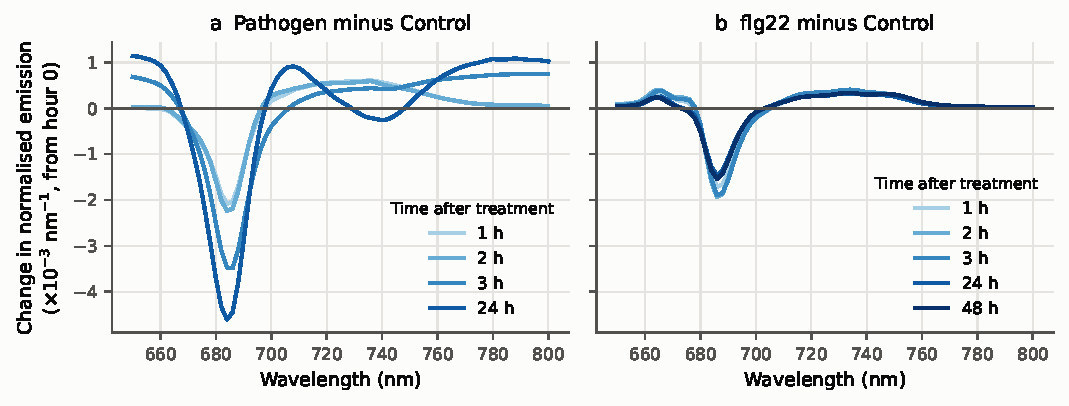
\includegraphics[width=\linewidth]{fig2_spectral_change.pdf}
\caption{\textbf{Treatment-induced change in emission-spectrum shape} (Col-0, set A;
area-normalised spectra, change from each plate's hour 0, treated minus Control).}
\label{fig:spectra}
\end{figure}

\begin{figure}[t]\centering
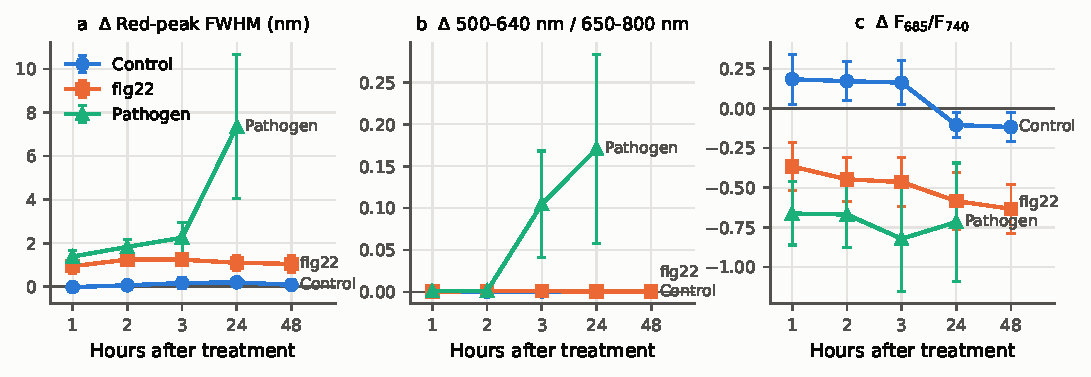
\includegraphics[width=\linewidth]{fig3_timecourse.pdf}
\caption{\textbf{Time course of three emission-shape features} (change from hour 0; mean
$\pm$ s.e.m. over plates). Data: \texttt{tables/fig3\_timecourse.csv}.}
\label{fig:time}
\end{figure}

\subsection{The flg22 signal does not depend on FLS2}
After baseline adjustment, flg22 plates were separable from Control plates at 1--3\,h
(AUC \aucFlgEarlyMin--\aucFlgEarlyMax{}; Fig.~\ref{fig:auc}b). With three plates per treatment
left, however, no result beat $p=\pFlgEarlyMin$ (\nPermFlgBase{} relabellings). The genetics
decide what this signal is. A model trained on Col-0 flg22-versus-Control shape features gave
an average flg22 score difference of \specFlgColO{} in Col-0 (out-of-fold, 1--3\,h),
\specFlgFlsSeventeen{} in \textit{fls2-17} and \specFlgFlsOneOhOne{} in \textit{fls2-101}
(Fig.~\ref{fig:spec}a). flg22 cannot act through FLS2 in the mutants, so this signal is a
property of the plates (handling, timing or seedling batch), not of flg22 perception. The
pathogen signature was likewise present in all genotypes (Fig.~\ref{fig:spec}b). This is
expected, because bacteria are perceived through patterns other than flagellin
\citep{zipfel2004}.

\begin{figure}[t]\centering
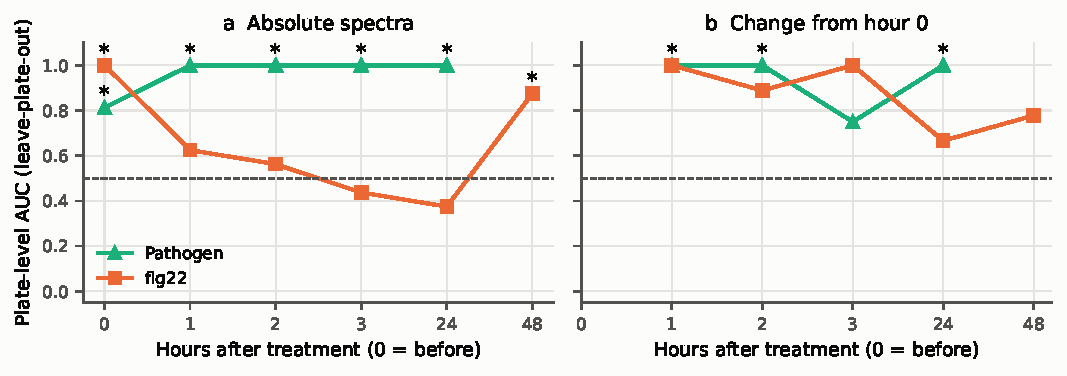
\includegraphics[width=\linewidth]{fig4_auc.pdf}
\caption{\textbf{Plate-level classification of treatment from spectra}, Col-0. (a) Absolute
spectra; hour~0 is before treatment. (b) Change from hour 0. * exact permutation $p\le0.05$.}
\label{fig:auc}
\end{figure}

\begin{figure}[t]\centering
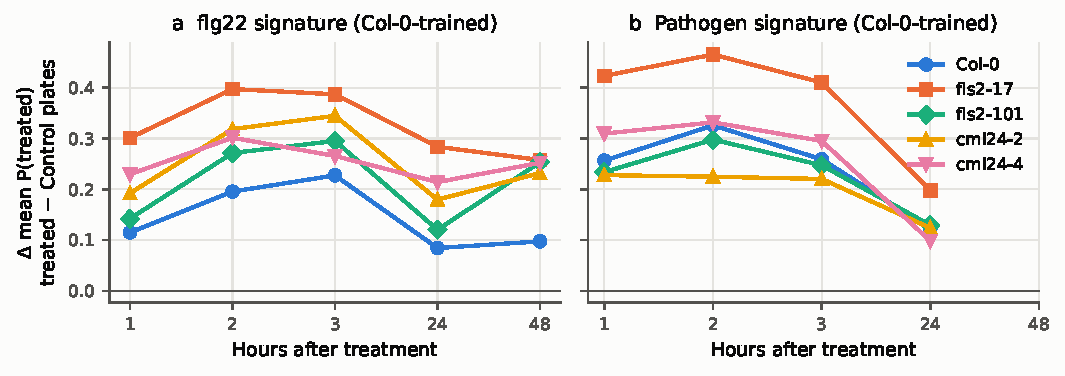
\includegraphics[width=\linewidth]{fig5_specificity.pdf}
\caption{\textbf{Genotype specificity of the signatures.} Col-0-trained model applied to each
genotype; difference in mean predicted probability between treated and Control plates.}
\label{fig:spec}
\end{figure}

\subsection{The independent replicate}
In the November replicate (set B; 405\,nm excitation), hand ROIs exist for one plate per
treatment, so treatment main effects cannot be separated from plate effects there. Within
plates, however, flg22 changed the emission shape of Col-0 differently from \textit{fls2-17}
at 6\,h (F$_{685}$/F$_{740}$ interaction $\setBinterSD$\,SD, $q=\setBinterq$; \setBinterN{}
related features). This is the pattern expected of FLS2-dependent perception. It was not seen
for \textit{fls2-101}. \pending{Plate-replicated set-B analysis from the raw cubes (2--3 plates
per treatment).}

\subsection{Seedling-level analysis of the raw cubes}
\pending{Segmentation of all cubes (Pathogen 48\,h, exposure-corrected intensity, spatial
heterogeneity) and pixel-level multivariate curve resolution \citep{dejuan2021}; label-transfer
validation in Supplementary Note 1.}

\section{Discussion}
Three lessons from this reanalysis apply beyond these data.
First, acquisition metadata must travel with hyperspectral intensities. A camera setting that
changed between timepoints produced the most striking pattern in the 2016 summaries.
Second, in plate-based seedling assays the plate, not the seedling, is the treated unit. Plates
can differ before treatment by as much as treatments differ afterwards, so a baseline image and
leave-plate-out validation are essential. Without them, a classifier here would have
``detected'' flg22 before it was applied.
Third, mutants that cannot perceive the stimulus are the decisive control. Here they showed that
an apparently promising flg22 signal was not perception.

What survives is a pathogen signature within 1--2\,h of inoculation: a broader red
emission peak and more short-wavelength emission. The timing is consistent with reports that
chlorophyll fluorescence changes precede visible symptoms \citep{bonfig2006}. Because the
signature appears in \textit{fls2} mutants, it does not require flagellin perception.
\pending{Whether CML24 modulates it awaits the seedling-level analysis; the hand-ROI data show
no cml24 $\times$ treatment interaction at $q<0.05$.}
\pending{Limitations: pathovar/strain, inoculum and seedling age unrecorded on the drive; four
plates per treatment; set-B excitation differs.}

% Methods. Every fact is traceable to ../metadata/FACTS_PENDING.md (source codes H, N, V1, V2,
% P, L) or to a script in ../scripts/. \pending{} marks facts still to be supplied.

\section{Methods}

\subsection{Plant material and treatments}
\textit{Arabidopsis thaliana} seedlings of five genotypes were grown on square agar plates in
five lanes per plate: Col-0 (lane A), \textit{fls2-17} (B), \textit{fls2-101} (C),
\textit{cml24-2} (D) and \textit{cml24-4} (E). Lane assignments are taken from the 2016 analysis
folders (FACTS R8). \pending{Allele origins, backgrounds and stock numbers.}
\textit{FLS2} encodes the flagellin receptor that perceives the flg22 epitope
\citep{gomezgomez1999,felix1999,gomezgomez2000,chinchilla2006}. \textit{CML24} encodes a
calmodulin-like Ca$^{2+}$ sensor \citep{delk2005} implicated in flg22-triggered nitric-oxide
signalling \citep{ma2008}.
Seedlings were grown for 7 days on 0.5$\times$ Murashige--Skoog/Linsmaier--Skoog basal salts with
0.1\% (w/v) sucrose and 0.5\,g\,L$^{-1}$ MES (pH 5.7), solidified with 0.8\% Phytagel (FACTS R21)
\pending{light, photoperiod and temperature}.
Plates were treated with a mock solution, flg22 (1\,$\mu$M, the laboratory's standard working
concentration; FACTS R17) or \textit{Pseudomonas syringae} pv.\ tomato DC3000 (FACTS R5, R16)
Bacteria were applied by flood inoculation after \citet{ishiga2011} at an OD$_{600}$ of 0.01 in
10\,mM MgCl$_2$ (FACTS R22). The 2016 protocol draft names Silwet L-77 as the mock
\pending{confirm mock and flg22 application method, FACTS P2}. Four plates per treatment were imaged in the July experiment (set A).

The independent November experiment (set B; FACTS R7, R9) used Col-0, \textit{fls2-17} and
\textit{fls2-101} only, with two or three plates per treatment, three rows per plate and three
seedlings per genotype per row. A pilot experiment (February--March 2016) measured rosette leaf
area from images of eight genotypes, including \textit{glr3.3} and \textit{glr3.4} alleles
(FACTS R10--R11). It is reported in the supplement only.

\subsection{Fluorescence hyperspectral imaging}
Plates were imaged in the Gilroy Laboratory (UW-Madison Botany) with a MacroPhor\texttrademark{}
fluorescence hyperspectral line-scan imager (Middleton Spectral Vision; FACTS R1). It carried an
Andor Zyla~5.5 sCMOS camera in 12-bit low-noise mode (FACTS R2). Set A used 488\,nm excitation
and 500--800\,nm emission (FACTS R3). The camera recorded 324 bands from 400.3 to 808.7\,nm at
about 1.23\,nm spacing. Set B used 405\,nm excitation and 400--800\,nm emission (FACTS R4),
recorded as 406 bands from 400.2 to 800.0\,nm, each row-scan acquired at two excitation laser powers,
50\% and 58\% of maximum (\texttt{Laser50}, \texttt{Laser58}; FACTS R15). Each plate was imaged as three
row-scans, one row of seedlings each.
Set A was imaged at \texttt{Hour0} (11:20--12:26 on 22 July 2016, about 6\,h before the 1\,h scans;
the pre-treatment baseline, FACTS R13) and at 1, 2, 3, 24 and
48\,h after infection (FACTS R6). Set B was imaged at 0, 6, 24 and 48\,h.
Acquisition settings were read from every ENVI header (\texttt{metadata/cube\_manifest.csv}).

\subsection{Data provenance and quality}\label{sec:quality}
All \nFiles{} files on the 2016 drive were inventoried and hashed (\texttt{scripts/00\_inventory.py}).
Every file name was parsed without exception: \nCubes{} hyperspectral cubes (\nCubesA{} set-A
samples, \nCubesB{} set-B samples, plus set-B bacteria-only and reference scans and one reference
and one artefact scan in set A) and \nRoiFiles{} hand-drawn region-of-interest (ROI) spectra
(\nRoiUnique{} unique by content hash). All \nShaRaw{} raw cubes carry SHA-256 checksums in
\texttt{metadata/cube\_manifest.csv}. We found the following problems and corrected for each where possible.
\begin{enumerate}
  \item \textbf{Exposure time changed between timepoints.} It was 0.305\,s at \texttt{Hour0},
  0.203\,s at 1--3\,h, 0.222--0.268\,s at 24\,h (varying within plates) and 0.222\,s at 48\,h.
  The 2016 summary graphs plotted uncorrected intensities, so their apparent drop between 0 and
  1\,h (about 1.5-fold) matches the exposure ratio $0.305/0.203=1.50$. We divide every intensity
  by its own exposure time, and our primary features are exposure-independent ratios
  (Section~\ref{sec:features}).
  \item \textbf{\texttt{Hour0} plates were scanned ``inverted''}, i.e.\ upside down (FACTS R14), except four
  rescans labelled ``NI'' made later the same day at the 1\,h settings. \texttt{Hour0} is used
  only as a baseline and is analysed separately from the upright timepoints.
  \item \textbf{Detector saturation.} At the \texttt{Hour0} exposure, up to
  \satHzeroMaxPct\% of a cube's seedling pixels (median \satHzeroMedPct\%) reached the 12-bit ceiling
  (4095 counts). Saturated pixels
  are excluded from all spectra.
  \item \textbf{Fixed scan order.} Within each timepoint plates were scanned Pathogen, then
  flg22, then Control, 20--40\,min apart, so scan time is partly confounded with treatment. We
  report the drift of Control plates between consecutive hours as a bound on this effect.
  \item \textbf{The plate is the experimental unit.} Treatments were applied per plate (four per
  treatment in set A), so treatment effects are tested at plate level. Genotype contrasts are
  within plates.
  \item \textbf{Inconsistent dark subtraction in the 2016 exports.} \nOffsetRoi{} hand-ROI spectra
  (Pathogen 3\,h plates 1--2 and 24\,h plate 4) were exported with the camera dark level
  (median \offsetMedian{} counts) still in them; all others were dark-subtracted (median
  \offsetCleanMedian{} counts). Because nothing fluoresces at wavelengths shorter than the
  excitation, each spectrum's mean below the excitation line (420--470\,nm in set A, 400--404\,nm
  in set B) was subtracted from it before features were computed (\texttt{scripts/01\_import\_rois.py}).
  \item \textbf{Missing cells.} No hand ROIs were drawn for Pathogen plates at 48\,h, although
  the cubes exist. Our automated segmentation covers them.
\end{enumerate}

\subsection{Spectral processing}\label{sec:features}
Each raw cube was read once, sequentially, and hashed with SHA-256
(\texttt{scripts/02\_harvest\_cubes.py}). The per-band dark level was taken as the median of
background pixels, which sit at about 108 counts. Seedlings were segmented on the dark-subtracted
685\,nm image at 10 background standard deviations, then cleaned, and cotyledon and hypocotyl
components were grouped (\texttt{src/pathofluor/segment.py}). Each segmented seedling was
assigned its lane and plant number from the row layout, which was validated against the 2016
hand ROIs (Supplementary Note~1). Spectral features were computed from the mean unsaturated
spectrum of each seedling after Savitzky--Golay smoothing (\texttt{src/pathofluor/features.py}):
\begin{itemize}
  \item the red/far-red ratio $F_{685}/F_{740}$ \citep{buschmann2007};
  \item the position and full width at half maximum of the red emission peak;
  \item the spectral centroid;
  \item the far-red fraction of 650--800\,nm emission;
  \item the short-wavelength fraction (500--640\,nm emission relative to 650--800\,nm), which
  captures the broad autofluorescence reported by the 2016 vendor analysis;
  \item exposure-normalised intensities (counts\,s$^{-1}$);
  \item per-pixel heterogeneity of the ratio and of the short-wavelength fraction.
\end{itemize}

\subsection{Statistics and classification}
\emph{Hand-ROI features (primary).} For each set, hour and feature we fitted
$y \sim \mathrm{treatment}\times\mathrm{genotype} + (1\,|\,\mathrm{plate})$ with Control and Col-0 as
references (\texttt{statsmodels} MixedLM, REML; features standardised), both on absolute values and
on change from the same plate and genotype at hour~0 (plates Control-4 and flg22-2 excluded from
the latter). $p$-values were adjusted by the Benjamini--Hochberg procedure across all features,
hours and contrasts within a set \citep{benjamini1995} (\texttt{scripts/05\_stats.py}).
\emph{Seedling-level features.} Seedling values were averaged per plate (and per plate and
genotype), expressed as change from hour~0, and compared between treated and Control plates by
Welch's $t$-test, or by the same mixed model for genotype interactions, with the same FDR control
(\texttt{scripts/05c\_seedling\_stats.py}).
\emph{Classification.} Logistic regression (L2, $C=0.1$) and PLS-DA (three components) on the
area-normalised spectrum or on the six shape features were evaluated by leave-one-plate-out
cross-validation. AUC was computed on plate means of out-of-fold scores. Significance came from an
exact permutation test that re-ran the whole cross-validation for every assignment of the treated
label to the same number of plates (\texttt{scripts/06\_models.py}).
\emph{Curve resolution.} MCR-ALS with three non-negative components was fitted to 1,500 unsaturated
seedling pixels per set-A cube (500--800\,nm, dark-subtracted, divided by exposure), initialised
from the purest pixels (\texttt{scripts/05b\_mcr.py}).

\subsection{Data and code availability}
Code (MIT licence), derived data, the 2016 hand-ROI spectra and all manifests are in the
repository. Raw cubes are deposited on Zenodo \pending{DOIs}. The two 2016 Middleton Spectral Vision
analysis reports \citep{msv2016july,msv2017nov} are cited but not redistributed (FACTS R19). The metadata follow MIAPPE where
applicable \citep{papoutsoglou2020} and the FAIR principles \citep{wilkinson2016}.


\section*{Acknowledgements}
\pending{Acknowledgements and funding (FACTS P10).}

\bibliographystyle{unsrtnat}
\bibliography{references}
\end{document}
